\documentclass[aspectratio=169,usenames,dvipsnames]{beamer}
\beamertemplatenavigationsymbolsempty
% \documentclass{beamer}

% UNCOMMENT FOR HANDOUTS
% \usepackage{pgfpages}
% \pgfpagesuselayout{2 on 1}[landscape,letterpaper,border shrink=5mm]
% \setbeameroption{show notes}

\mode<presentation>
\usetheme{Boadilla}
\usecolortheme{spruce}
\usepackage{../../LizStyle,ulem}
\usepackage{color}
\usepackage[color,matrix,arrow]{xy}
% \input xy
% \xyoption{all}
\usepackage{tikz}
\usepackage{tikz-cd}
\tikzset{commutative diagrams/diagrams={ampersand replacement=\&}}

\AtBeginSection{\frame{\sectionpage}}


% ==========Command for putting comments and removing them=======
% Visible:
\newcommand{\InstructorNotes}[1]{\textit{\color{orange}#1}}
\newcommand{\InstructorList}[1]{
\begin{itemize}
	\color{orange}
	#1
\end{itemize}
}
% Removed:
\renewcommand{\InstructorNotes}[1]{}
\renewcommand{\InstructorList}[1]{}


\newcommand{\bvfill}{\vskip0pt plus 1filll}

\usepackage{multimedia}
\usepackage{graphbox}

% \usepackage{algpseudocode}


\newcommand{\Reeb}{\textbf{Reeb}}
\newcommand{\Rtopc}{\textbf{Rtopc}}
% \newcommand{\RR}{\mathcal{R}}

\newcommand{\Set}{\textbf{Set}}
\newcommand{\Vect}{\textbf{Vect}}
\newcommand{\Top}{\textbf{Top}}
\newcommand{\Int}{\textbf{Int}}


\graphicspath{ {Figures/} {../Figures/}{../../Figures/} }



\begin{document}
%\pdfoptionpdfminorversion 5
%\logo{\includegraphics[height=1.5cm]{dukeshield.pdf}}
\title[]{Ch 5.1.4-5: More Cross-Validation}
\subtitle{Lecture 14 - CMSE 381}
\date{Wed, Feb 18, 2026}



\institute[MSU-CMSE]{Michigan State University\\
			::\\
          Dept of Computational Mathematics, Science \& Engineering}


\begin{frame}
 \titlepage


\end{frame}
%--------------------------
\begin{frame}[c]{Announcements}

\begin{columns}
\column{.45\textwidth}
\centering

	\textbf{Last time:}
	\begin{itemize}
		\item k-fold CV
	\end{itemize}
	\textbf{This lecture:}
	\begin{itemize}
		\item More $k$-fold CV
		\item Bias-Variance Tradeoff
		\item CV for classification
	\end{itemize}

	% \textbf{Announcements:}
	% \begin{itemize}
	% 	\item Exam 1 feedback sent
	% \end{itemize}
\column{.45\textwidth}
\centering
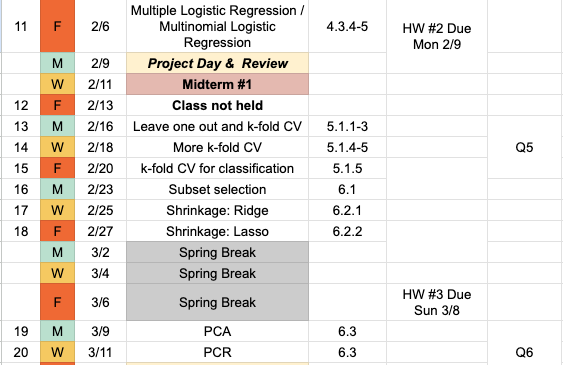
\includegraphics[alt={Screenshot of the course schedule for lectures 11 to 20.},width = \textwidth]{Schedule-S26-Lecs11_to_20}
\end{columns}

\end{frame}
%--- Next Frame ---%

%=================
\section{$k$-fold CV}
%=================

\begin{frame}[t]{Approximations of Test Error}
\begin{columns}
\column{.3\textwidth}
\centering
\textbf{Validation Set}
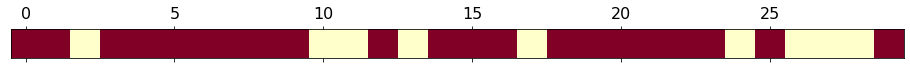
\includegraphics[alt={Diagram showing the first validation set split.},width = \textwidth]{CV-subset0}
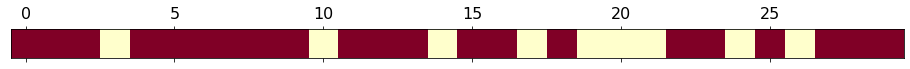
\includegraphics[alt={Diagram showing the second validation set split.},width = \textwidth]{CV-subset1}
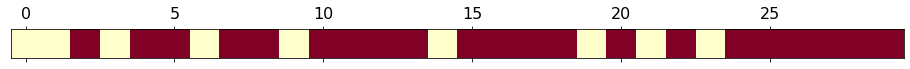
\includegraphics[alt={Diagram showing the third validation set split.},width = \textwidth]{CV-subset2}
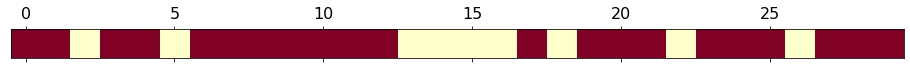
\includegraphics[alt={Diagram showing the fourth validation set split.},width = \textwidth]{CV-subset3}
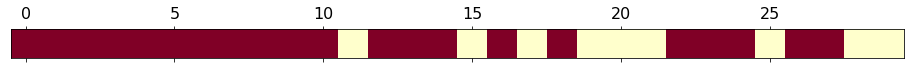
\includegraphics[alt={Diagram showing the fifth validation set split.},width = \textwidth]{CV-subset4}
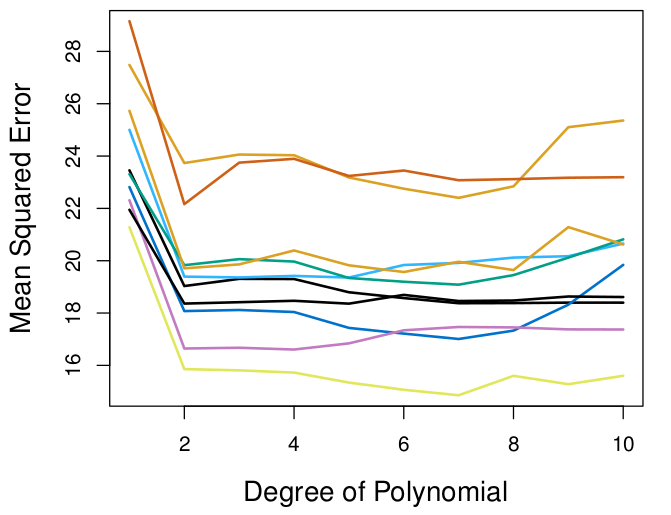
\includegraphics[alt={Figure labeled validation set for comparison.},width = .8\textwidth]{Fig5-2b}
\column{.3\textwidth}
\centering
\textbf{LOOCV}
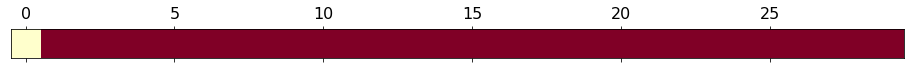
\includegraphics[alt={Diagram showing the first leave-one-out cross-validation split.},width = \textwidth]{LOOCV-subset0.png}

\includegraphics[alt={Diagram showing the second leave-one-out cross-validation split.},width = \textwidth]{LOOCV-subset1.png}

\includegraphics[alt={Diagram showing the third leave-one-out cross-validation split.},width = \textwidth]{LOOCV-subset2.png}
% 
\includegraphics[width = \textwidth]{LOOCV-subset3.png}
% 
\includegraphics[width = \textwidth]{LOOCV-subset4.png}
$\vdots$

\includegraphics[alt={Diagram showing the final leave-one-out cross-validation split.},width = \textwidth]{LOOCV-subset29.png}
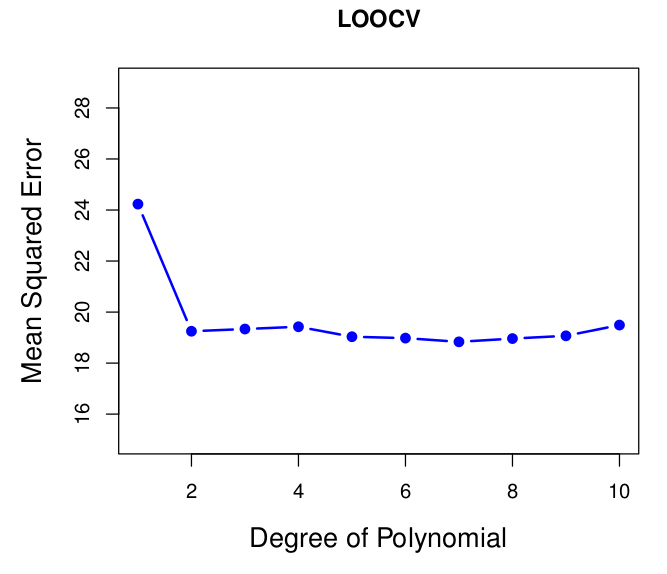
\includegraphics[alt={Figure using the auto data example to show a fixed result with no randomness across repeated runs.},width = .8\textwidth]{Fig5-4a}

\column{.3\textwidth}
\centering
\textbf{K-fold CV}
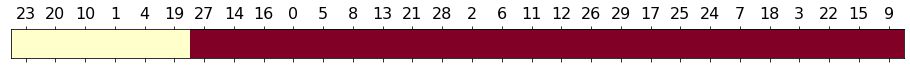
\includegraphics[alt={Diagram showing the first split in five-fold cross-validation.},width = \textwidth]{CV-Kfold-subset0}

\includegraphics[alt={Diagram showing the second split in five-fold cross-validation.},width = \textwidth]{CV-Kfold-subset1}

\includegraphics[alt={Diagram showing the third split in five-fold cross-validation.},width = \textwidth]{CV-Kfold-subset2}

\includegraphics[alt={Diagram showing the fourth split in five-fold cross-validation.},width = \textwidth]{CV-Kfold-subset3}

\includegraphics[alt={Diagram showing the fifth split in five-fold cross-validation.},width = \textwidth]{CV-Kfold-subset4}
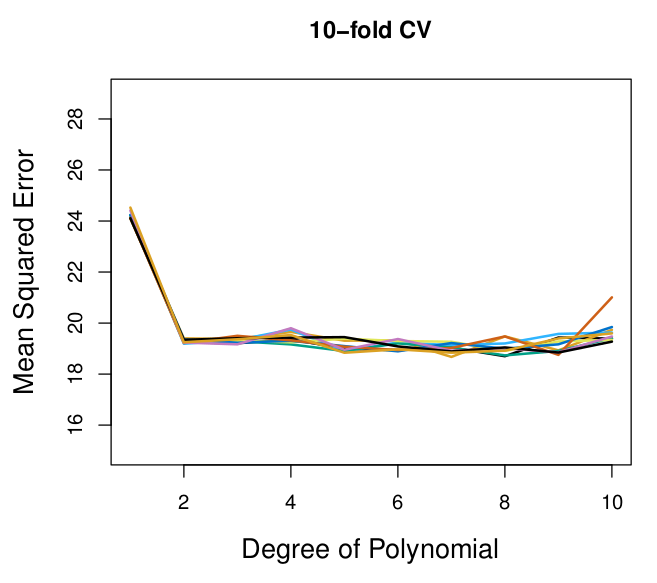
\includegraphics[alt={Second figure from the auto data example.},width = .8\textwidth, align = c]{Fig5-4b}
\end{columns}
\end{frame}
%--- Next Frame ---%



%--- Next Frame ---%
\begin{frame}[c]{Definition of $k$-fold CV}

\begin{columns}
\column{.45\textwidth}
\centering
\begin{itemize}
	\item Randomly split data into $k$-groups (folds)
	\item Approximately equal sized. For the sake of notation, say each set has $\ell$ points
	\item []
	\item Remove $i$th fold $U_i$ and reserve for testing.
	\item Train the model on remaining points
	\item Calculate $\mathrm{MSE}_i = \frac{1}{\ell} \sum_{(x_j,y_j) \in U_i}(y_j-\hat y_j)^2$
	\item[]
	\item Rinse and repeat
\end{itemize}
\column{.45\textwidth}
\centering
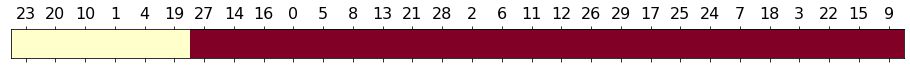
\includegraphics[alt={Diagram showing the first split in five-fold cross-validation.},width = \textwidth]{CV-Kfold-subset0}

\includegraphics[alt={Diagram showing the second split in five-fold cross-validation.},width = \textwidth]{CV-Kfold-subset1}

\includegraphics[alt={Diagram showing the third split in five-fold cross-validation.},width = \textwidth]{CV-Kfold-subset2}

\includegraphics[alt={Diagram showing the fourth split in five-fold cross-validation.},width = \textwidth]{CV-Kfold-subset3}

\includegraphics[alt={Diagram showing the fifth split in five-fold cross-validation.},width = \textwidth]{CV-Kfold-subset4}
Return
\begin{equation*}
	CV_{(k)} = \frac{1}{k} \sum_{i=1}^k \mathrm{MSE}_i
\end{equation*}
\end{columns}

\end{frame}
%--- Next Frame ---%

%--- Next Frame ---%
\begin{frame}[t]{Comparison with simulated data: Ex 3}

\begin{columns}
\column{.35\textwidth}
\centering
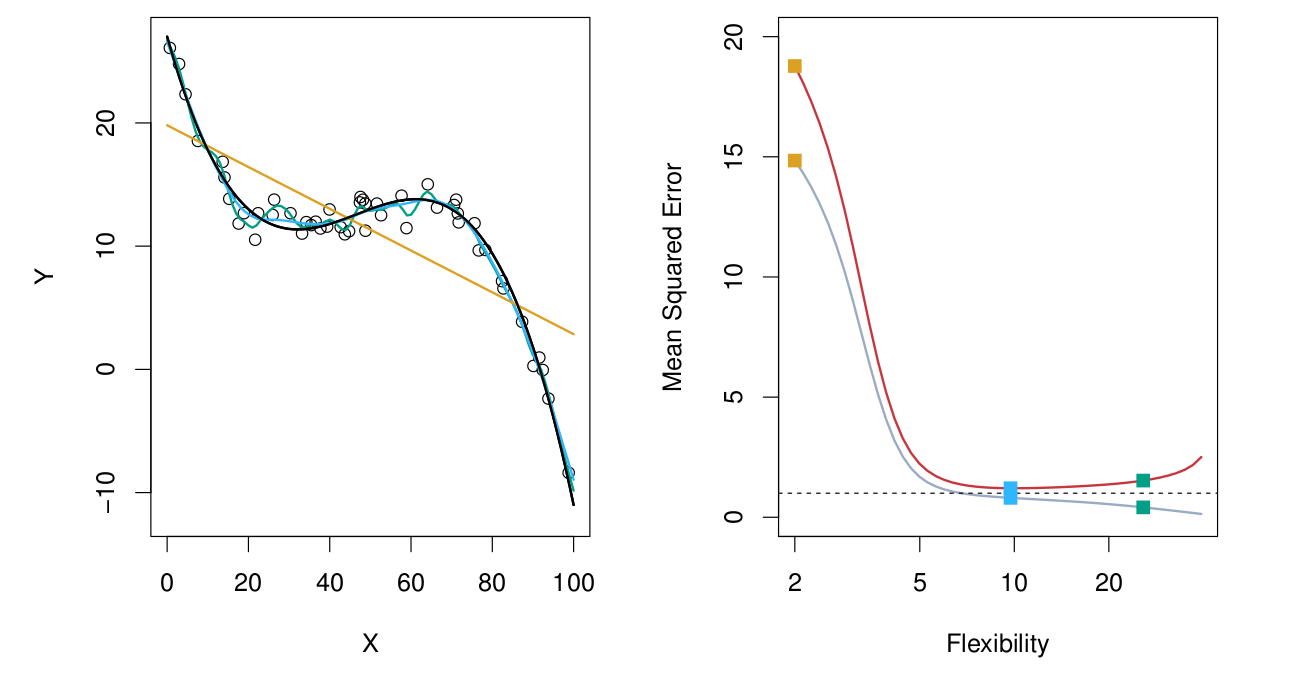
\includegraphics[alt={Plot of simulated nonlinear data with fitted curves of different flexibility and corresponding error behavior.},width = \textwidth, align = c, trim = 0 0 700 0, clip]{Fig2-11}
\column{.3\textwidth}
\centering
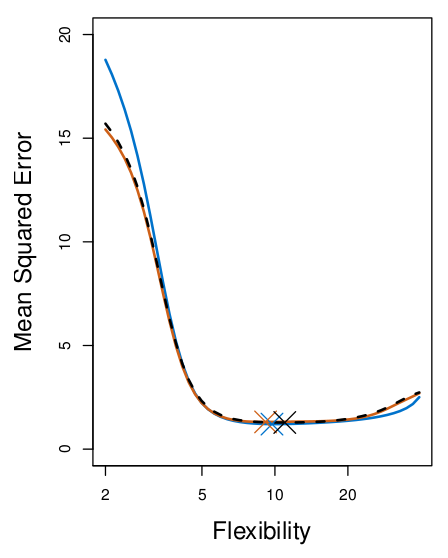
\includegraphics[alt={Plot comparing true test MSE, LOOCV estimate, and 10-fold cross-validation estimate, showing very similar results.},width = \textwidth, align = c]{Fig5-6c}
\column{.3\textwidth}
\InstructorNotes{}
\InstructorList{
  \item Blue: true test MSE is shown in   blue
  \item Black dashed:  the LOOCV estimate 
  \item Orange: 10-fold CV 
  \item The crosses indicate the minimum of each of the   MSE curves.
  \item Nearly the same
}


\end{columns}
\InstructorNotes{}
\end{frame}
%--- Next Frame ---%
\begin{frame}[t]{Comparison with simulated data: Ex 1}

\begin{columns}
\column{.35\textwidth}
\centering
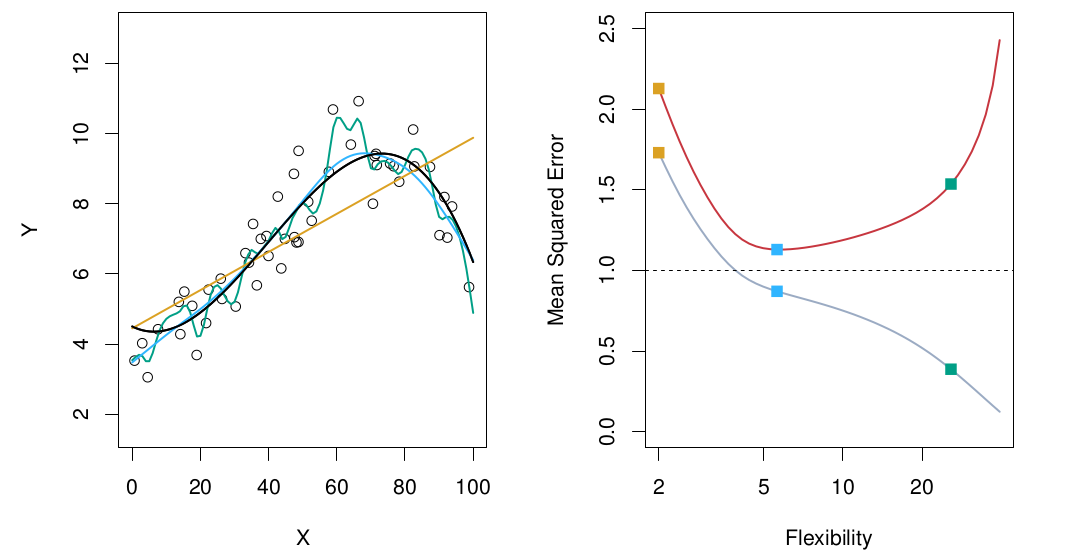
\includegraphics[alt={Plot of simulated nonlinear data with fitted curves of different flexibility and corresponding training and test error behavior.},width = \textwidth, align = c, trim = 0 0 590 0, clip]{Fig2-9}
\column{.32\textwidth}
\centering
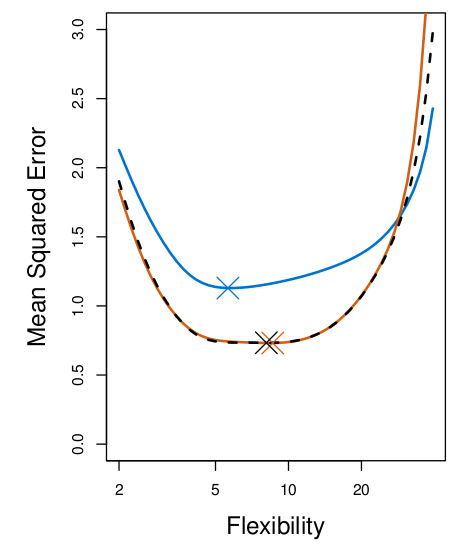
\includegraphics[alt={Plot comparing true test MSE, LOOCV estimate, and 10-fold cross-validation estimate, showing that the cross-validation estimates underestimate the true test MSE.},width = \textwidth, align = c]{Fig5-6a}

\column{.3\textwidth}
\InstructorList{
  \item Blue: true test MSE is shown in   blue
  \item Black dashed:  the LOOCV estimate 
  \item Orange: 10-fold CV 
  \item The crosses indicate the minimum of each of the   MSE curves.
  \item \textbf{Underestmates the true test MSE}
}
\end{columns}
\end{frame}
%--- Next Frame ---%
\begin{frame}[t]{Comparison with simulated data: Ex 2}

\begin{columns}
\column{.35\textwidth}
\centering
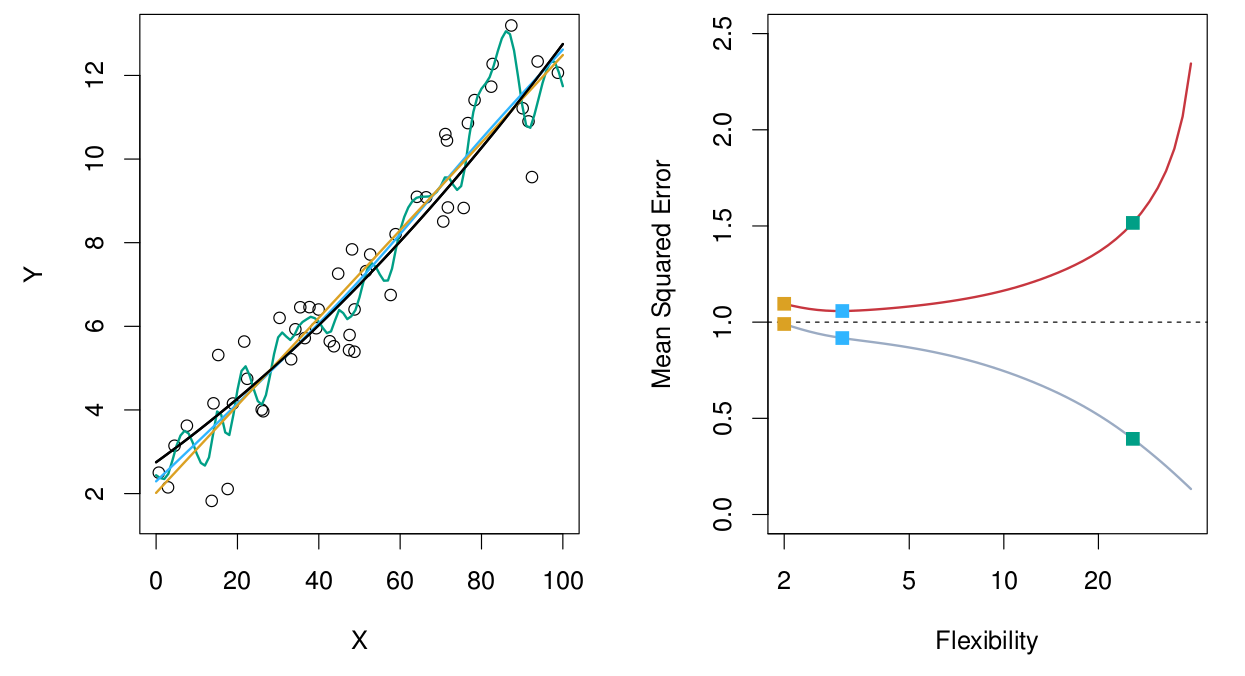
\includegraphics[alt={Plot of simulated close-to-linear data with fitted curves of different flexibility and corresponding training and test error behavior.},width = \textwidth, align = c, trim = 0 0 600 0, clip]{Fig2-10}
\column{.29\textwidth}
\centering
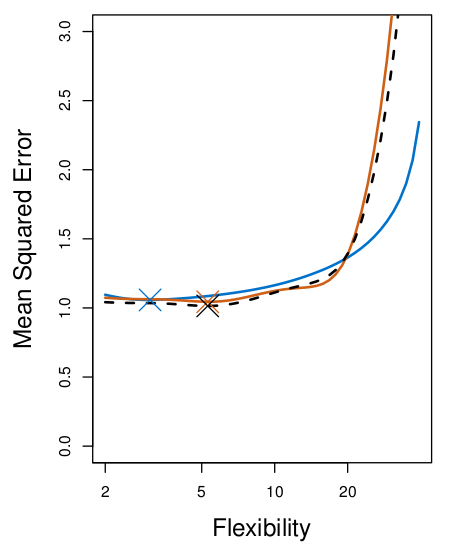
\includegraphics[alt={Plot comparing true test MSE, LOOCV estimate, and 10-fold cross-validation estimate, showing close agreement at low flexibility and overestimation at higher flexibility.},width = \textwidth, align = c]{Fig5-6b}
\column{.29\textwidth}
\InstructorNotes{Close for lower flexibility, then overestimates at higher ranges}

\end{columns}
\end{frame}
%--- Next Frame ---%
\begin{frame}[c]{Takeaways from the examples}

\begin{columns}
\column{.45\textwidth}
\centering
\InstructorList{
\item In all plots, LOOCV and 10-fold CV are similar
\item Sometimes really only care about the minimum point in the test MSE because want to get the right degree of freedom for a model. All examples have approximately same x-coord for that

}
\column{.45\textwidth}
\centering

\end{columns}

\end{frame}
%--- Next Frame ---%
\begin{frame}[t]{Bias-Variance Tradeoff: Bias}
	\begin{equation*}
		E(y_0 - \hat f (x_0))^2 = \Var(\hat f (x_0))
			+ \left[\mathrm{Bias}(\hat f(x_0)) \right] ^2
			+ \Var(\e)
	\end{equation*}
\begin{columns}
\column{.45\textwidth}
\centering
% \textbf{Bias}
\InstructorList{
\item note we talk about bias in estimation of test error rate
\item 1.... Validation set overestimates test error b/c used small subset of data
\item 3.... $k$-fold gives medium level of bias b/c training set has approximately $(k-1)n/k$ observations
\item 2....LOOCV gives approximately unbiased estimate since uses almost all data every time
}
\column{.45\textwidth}
\centering
\InstructorList{
\item sooooooooo LOOCV better than $k$-fold just for bias
}
\end{columns}

\end{frame}
%--- Next Frame ---%
\begin{frame}[t]{Bias-Variance Tradeoff: Variance}
	\begin{equation*}
		E(y_0 - \hat f (x_0))^2 = \Var(\hat f (x_0))
			+ \left[\mathrm{Bias}(\hat f(x_0)) \right] ^2
			+ \Var(\e)
	\end{equation*}
\begin{columns}
\column{.45\textwidth}
\centering

% \textbf{Variance}
\InstructorList{
\item note we talk about variance in estimation of test error rate

\item LOOCV higher variance:
\InstructorList{
	\item avg the outputs of n fitted models, but all on almost identical observations
	\item high correlation with each other
	\item repeated measure problem in science! - don't generalize well across samples
}

}

\column{.45\textwidth}
\centering
\InstructorList{
\item $k$-fold
\InstructorList{
	\item $k$ fitte models somewhat less correlated with each other
	\item mean of many highly correlated quantities has higher variance than those not corrleated
}
\item Empirically, $k=5$ or 10 has been shown to be a happy medium
}
\end{columns}

\end{frame}
%--- Next Frame ---%
% %--- Next Frame ---%
% \begin{frame}[t]{Bias-Variance Tradeoff}
% 	{Added frame from later slide deck, might want to incorporate}
% 	\begin{equation*}
% 		E(y_0 - \hat f (x_0))^2 = \Var(\hat f (x_0))
% 			+ \left[\mathrm{Bias}(\hat f(x_0)) \right] ^2
% 			+ \Var(\e)
% 	\end{equation*}
% \begin{columns}
% \column{.45\textwidth}
% \centering
% \textbf{Higher Bias}
% \begin{itemize}
% \item Validation set overestimates test error b/c used small subset of data
% \item $k$-fold gives medium level of bias b/c training set has approximately $(k-1)n/k$ observations
% \item LOOCV gives approximately unbiased estimate since uses almost all data every time
% \end{itemize}

% \textbf{Lower Bias}
% \column{.45\textwidth}
% \centering
% \textbf{Higher Variance}
% \begin{itemize}
% \item LOOCV: avg the outputs of $n$ fitted models with high correlation
% \item $k$-fold: $k$ fitted models somewhat less correlated with each other
% \end{itemize}

% \textbf{Lower Variance}
% \end{columns}
% \centering
% {\color{violet}
% Usually use $k=5$ or $k=10$
% }
% \end{frame}

% --- Next Frame --- %
\begin{frame}[c]{In short: Vadidation vs Test}
	\begin{itemize}
		\item all the time, we are pretending the validation set etc is the test set...
		\item when it is not. 
	\end{itemize}

\InstructorList{
	\item a true test set is an independent sample
	\item CV measures will never achieve that
}
\end{frame}

 --- Next Frame --- %
\begin{frame}[c]{Real-world example: Chekroud et al., Science 383, 164–167 (2024) }
	\centering
	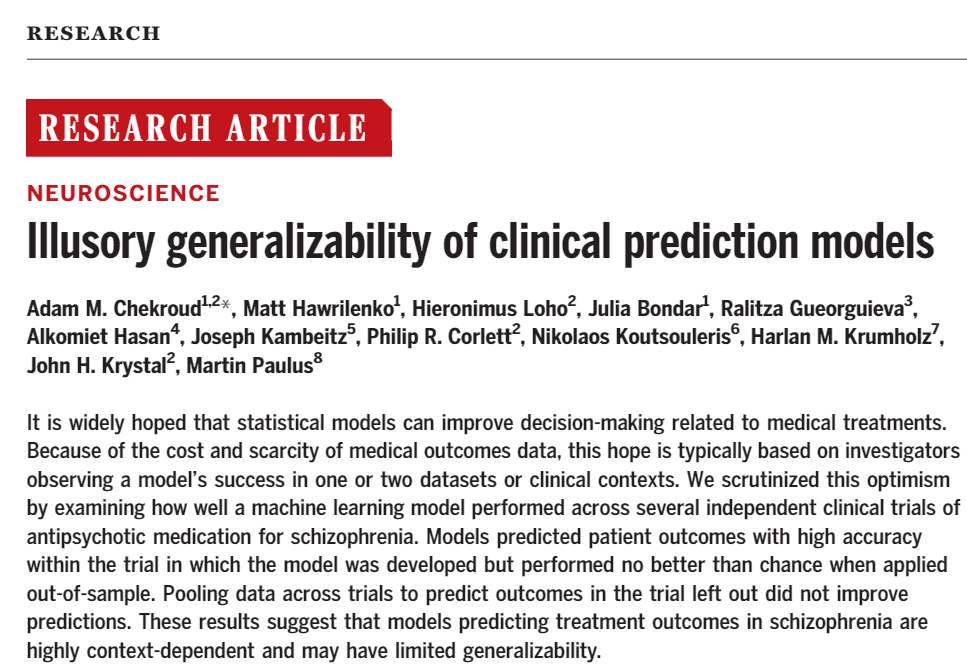
\includegraphics[alt={Figure from a real-world example in Chekroud et al., Science 383, 164–167 (2024).},width=0.7\textwidth]{illusory_generalizability_science2024_1.png}
	
\end{frame}

% --- Next Frame --- %
\begin{frame}[c]{Real-world example: Chekroud et al., Science 383, 164–167 (2024) }
	\centering
	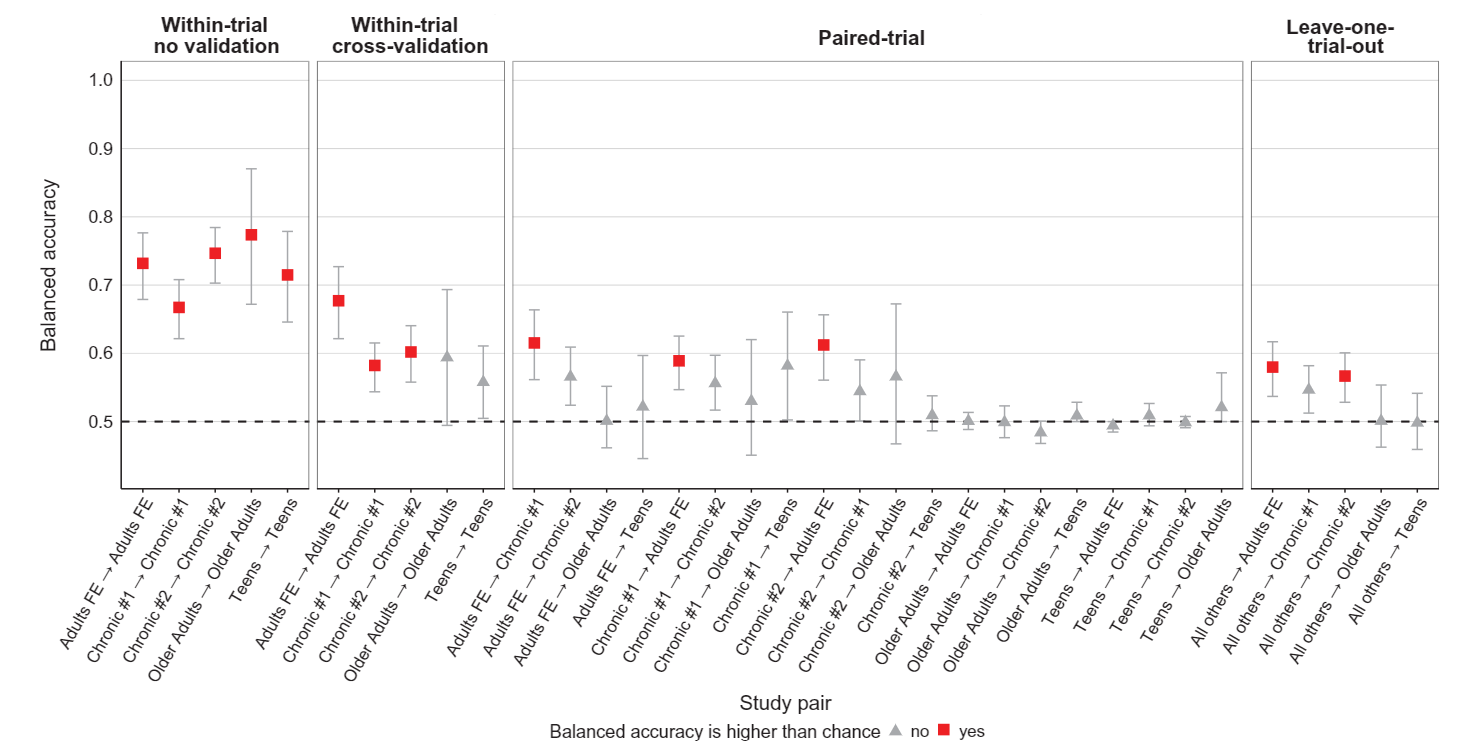
\includegraphics[alt={Second figure from a real-world example in Chekroud et al., Science 383, 164–167 (2024).},width=0.95\textwidth]{illusory_generalizability_science2024_2.png}
	
\end{frame}

% %--- Next Frame ---%
%=================
\section{Using K-Fold CV on Polynomial Linear Regression}
%=================

\begin{frame}[c]{Polynomial regression}

	\begin{columns}
	\column{.45\textwidth}
	\centering
	Replace linear model
	\begin{equation*}
		y_i = \beta_0 + \beta_1x_1 + \e_i
	\end{equation*}
	with
	\begin{equation*}
		y_i = \beta_0 + \beta_1x_1 + \beta_2x_1^2 + \cdots + \beta_dx_1^d + \e_i
	\end{equation*}
	
	\column{.45\textwidth}
	\centering
	\InstructorList{
	  \item Can learn with linear models by passing in predictors $x_i^\ell$
		\item Tend to not go higher than degree 3 or 4 because makes overly flexible
	}
	
	\end{columns}
\end{frame}
%--- Next Frame ---%
\begin{frame}[t]{Faking linear regression into doing our work for us}
\begin{columns}
\column{.45\textwidth}

\InstructorList{
  \item Draw a column of data 
  \item Draw the version with squares and cubes in the columns 
  \item Pass to linear regression and interpret the coefficients as the ones we want.
}

\centering
\column{.45\textwidth}
\centering
\end{columns}
\end{frame}
%--- Next Frame ---%

{
\setbeamercolor{background canvas}{bg=Apricot!25}
\begin{frame}[t]{Coding - Build a plot for train/test scores vs flexibility}
\begin{columns}
\column{.45\textwidth}
\centering
\column{.45\textwidth}
\centering
\end{columns}
\end{frame}
}
%--- Next Frame ---%


% %----------------
\begin{frame}[t]{Next time}

    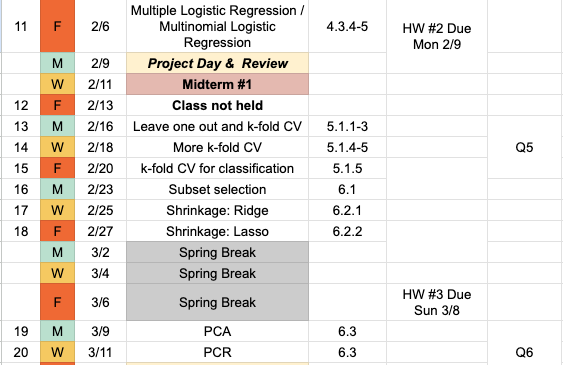
\includegraphics[alt={Screenshot of the course schedule for lectures 11 to 20.},align = c, width = .65\textwidth]{Schedule-S26-Lecs11_to_20}
\begin{columns}
\column{.45\textwidth}
\centering


\column{.45\textwidth}

\end{columns}
\end{frame}
%--- Next Frame ---%


\end{document}
